%(Aquí lo dejaría con la estructura que teníamos para Caise, presentamos el framework y posteriormente comentamos modelos y transformaciones)

In this section we present $\pi$SOD-M, an MDD-based methodology for building service compositions with non-functional requirements. 
$\pi$SOD-M extends SOD-M with concepts for modelling non-functional requirements.
$\pi$-SODM (Figure~\ref{fig:piSOD-M}) proposes the generation of a set of models at different levels of abstraction, as well as transformations between these models.
\begin{figure}[h]
\centering
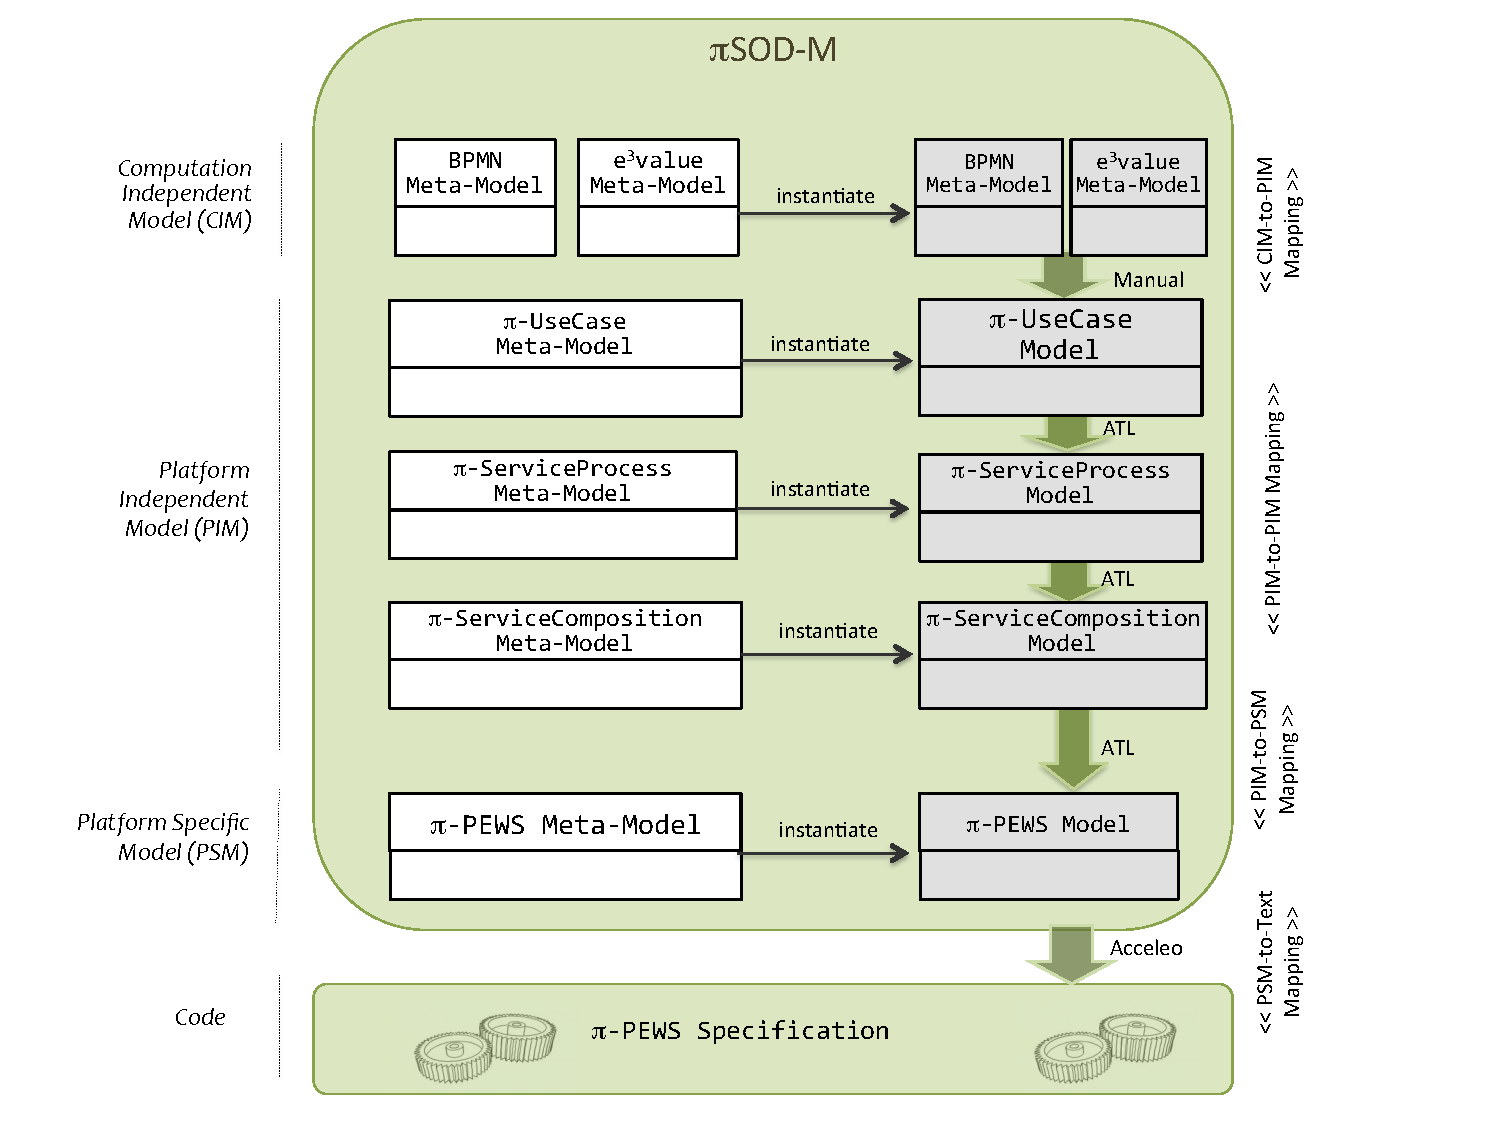
\includegraphics[width=1.0\textwidth]{figs/piSOD-M_process.pdf}
\caption{$\pi$SOD-M Overview.}
\label{fig:piSOD-M}
\end{figure}

$\pi$-SODM proposes meta-models, organized into three levels (Figure~\ref{fig:piSOD-M}): CIM (\textit{Computational Independent Models}), PIM (\textit{Platform Independent Models}) and PSM (\textit{Platform Specific Models}). 
These models are explained next.

\subsection{Computation Independent Models}

This level focusses on the highest-level view of the system, including its business and requirement specifications.
At this stage of the development, the structure and system processing details are still unknown or undetermined.  
$\pi$-SODM uses the \textit{e$^3$value}~\cite{e3value} and \textit{BPMN}~\cite{BPMN} meta-models for this purpose. 

The e$^3$value model identifies the value/information exchange between components of the system. 
It defines \textit{dependency paths}, showing the value exchanges, which are triggered by the occurrence of an end-consumer need.
A dependency path has a direction and consists of a sequence of linked dependency nodes.
A dependency path starts with a \textit{start stimulus} node and ends with an \textit{end stimulus} node\footnote{See Legend on Figure~\ref{fig:CIM:tpme3v}}. 
Dependency paths may also contain \textsl{OR} and \textsl{AND} elements (both for initiate and join alternative and parallel paths).

The BPMN model is a graphical representation that establishes the high-level workflow of the application.

The next example illustrates the use of these models.
\begin{example}[To Publish Music]\label{ex:toPublicMusic}
To illustrate our proposal, we build the models for a ``To Publish Music'' problem. 
This problem involves three external actors ({\em Spotify, Twitter} and {\em Facebook}), as well as the user and the application itself.

The e$^3$value and BPMN models for this applications are shown in Figure~\ref{fig:CIM:tpm}.
Notice that the models at this level show\dots 
{\color{red} Valeria and Placido: Please explain the CIM models for this example.}
%\hfill\openbox
\end{example}

\begin{figure}\center
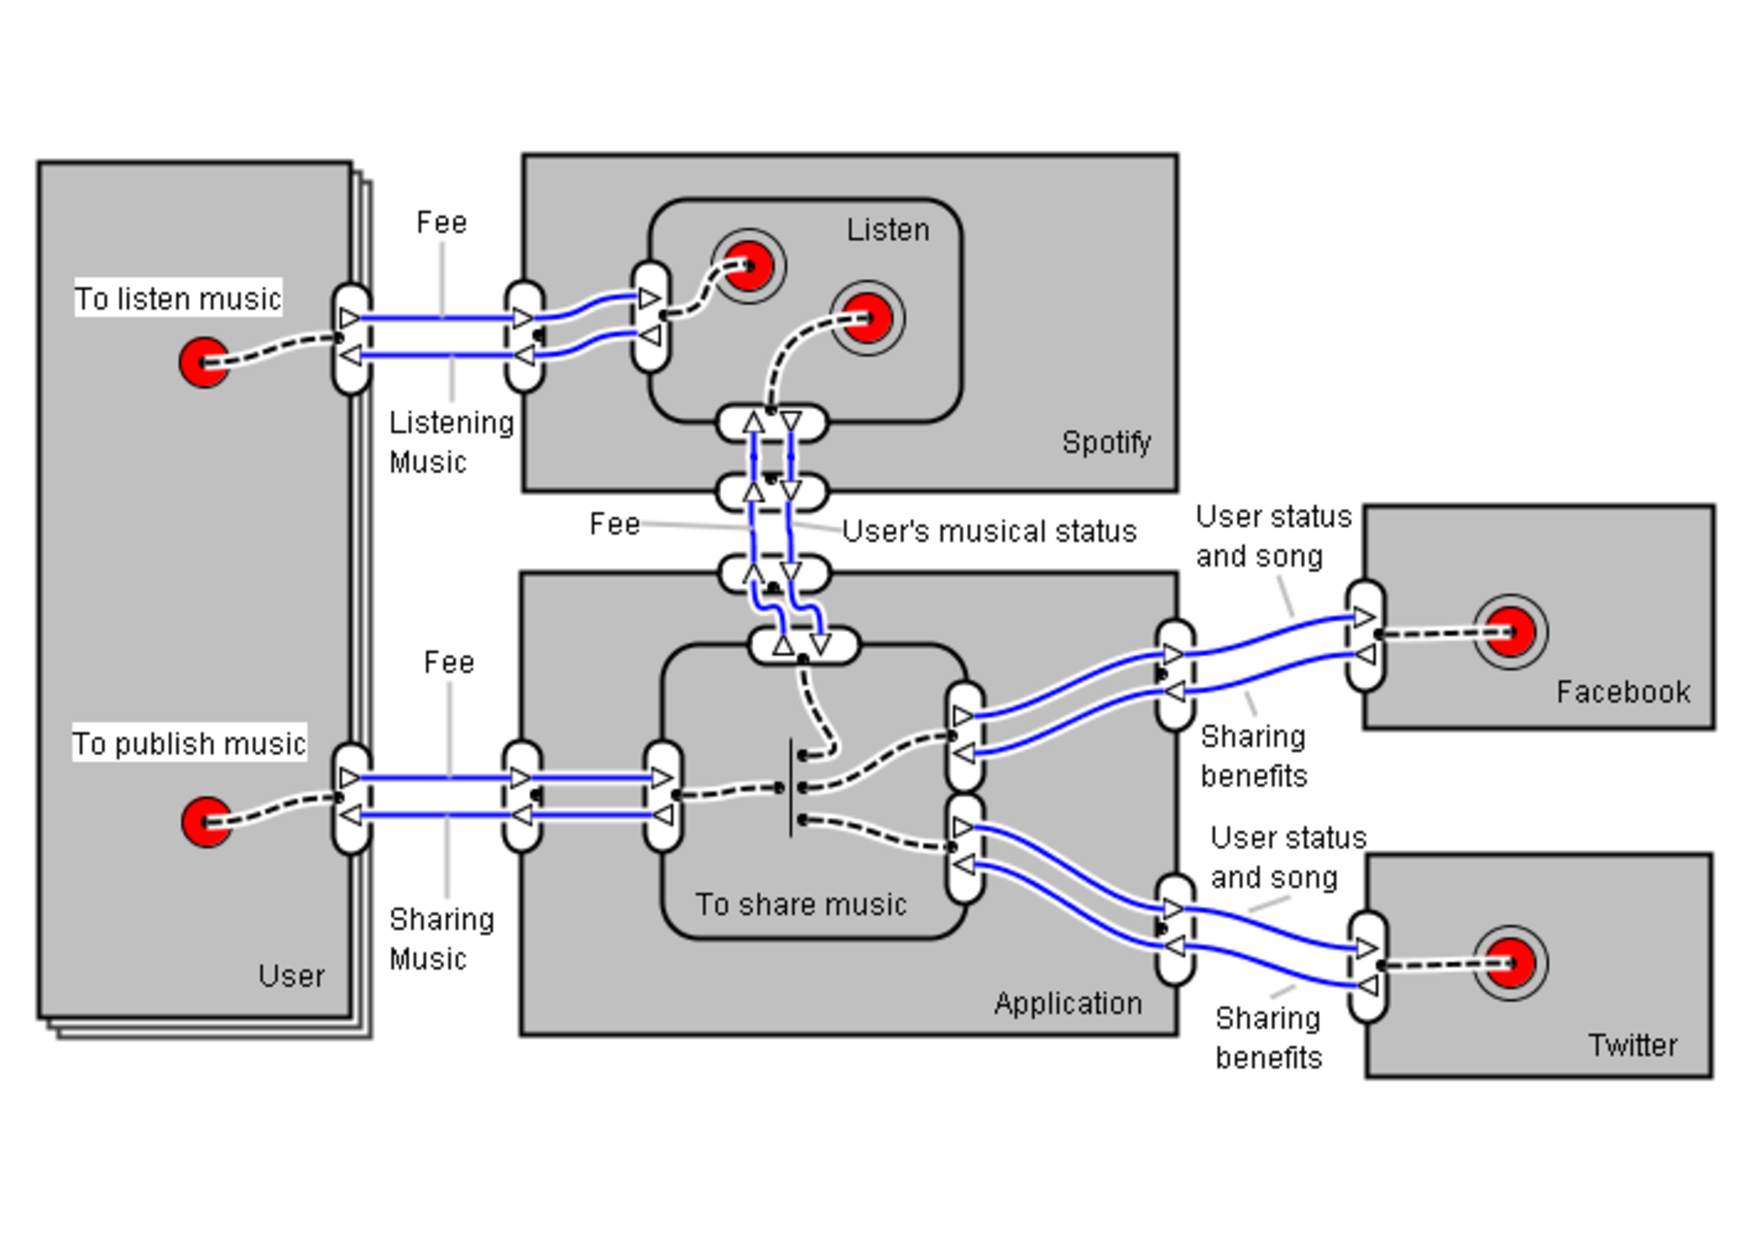
\includegraphics[width=0.88\textwidth]{figs/e3value.pdf}
\hspace*{5cm}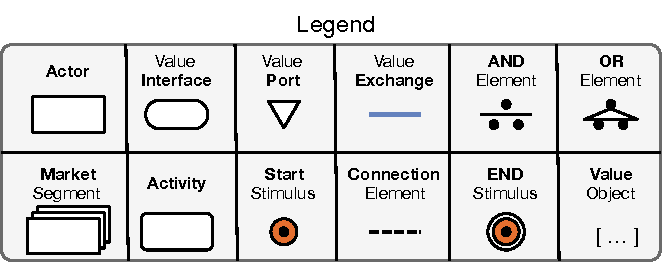
\includegraphics[width=0.4\textwidth]{figs/3ValueKey.pdf}
\caption{\label{fig:CIM:tpme3v} e3value model for ``To Publish Music''.}
\end{figure}

\begin{figure}\center
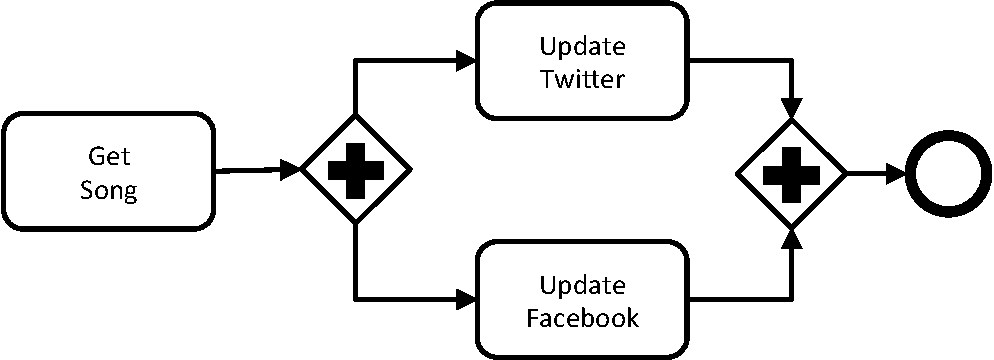
\includegraphics[width=0.49\textwidth]{figs/SC.pdf}
\caption{\label{fig:CIM:tpmbpmn} BPMN model for ``To Publish Music''.}
\end{figure}

The CIM level models are the basis for the development of the application. 
The information presented at this level are (manually) refined into PIM-level models.


\subsection{Platform Independent Models}

This level focusses on the system functionality, hiding the details of any particular platform.
The specification defines those parts of the system that do not change from one platform to another. 
Our method defines three PIM-level meta-models: \textit{$\pi$-UseCase}, \textit{$\pi$-ServiceProcess} and \textit{$\pi$-ServiceComposition}.
 
The \textit{$\pi$-UseCase} meta-model extends the UML Use Case meta-model for describing functional and non-functional requirements. 
Non-functional requirements are defined as \textit{constraints} over actions and data.

\begin{example}[To Publish Music \textit{(cont)}]\label{ex:toPublicMusic2}
{\color{red} Talk about this model for the example.}
\end{example}

 
The \textit{$\pi$-ServiceProcess} meta-model defines the concept of \textit{service contract} to represent constraints over data and actions 
gathers the constraints described in the \textit{$\pi$-UseCase}.

\begin{example}[To Publish Music \textit{(cont)}]\label{ex:toPublicMusic3}
{\color{red} Talk about this model for the example.}
\end{example}

The \textit{$\pi$-ServiceComposition} meta-model provides the concept  of \textit{Policy}
to integrate contracts with similar non-functional requirements.
For instance, security and privacy restrictions may be grouped into a security policy.


\begin{example}[To Publish Music \textit{(cont)}]\label{ex:toPublicMusic4}
We model a business process that consists of three service activities: {\em Listen Music}, {\em Publish Music} and {\em Confirmation}. 
The {\em Publish Music} activity calls the {\em Facebook} and {\em Twitter} services.
Both {\em Facebook} and {\em Twitter} require authentication. 
Two authentication policies are required, one for {\em Twitter} and another for {\em Facebook}.
{\color{red} To be completed!.}
\end{example}

\subsection{Platform Specific Models}

This level focusses on the functionality, in the context of a particular implementation platform.
Models at this level combine the platform-independent view with the specific aspects of the platform to implement the system. At the PSM level we have lower-level models that can be automatically translated into actual computer programs. 
We have defined one meta-model at this level.

The \textit{$\pi$-PEWS} meta-model provides concepts for modelling service compositions. 
Instances of this meta-model are textual descriptions of service compositions that can be translated into any service composition language, such as BPEL~\cite{bpel03} or PEWS~\cite{BaCAM05,Placido2010LTPD}.

PEWS~\cite{BHM06,Placido2010LTPD} is a notation to express service compositions.
The language is based on the notion of Path Expressions~\cite{And79} and can easily be translated into any actual composition language, such as BPEL~\cite{bpel03} or any other language that lets the service designer combine the methods or subprograms that implement each operation of a service, in order to achieve the desired application logic. 
Figure~\ref{fig:metamodel} presents the $\pi$-{\sc Pews} meta-model, where we identify classes to describe:
\begin{itemizedTrivlist}
\item Service compositions: {\sc Namespace} representing the interface exported by a service, {\sc Operation} that represents a call to a service method, {\sc CompositeOperation}, {\sc Operator} and {\sc Path} for representing service compositions.
A {\sc Path} can be an {\sc Operation} or a {\sc Compound Operation}. 
A {\sc Compound Operation} is defined using an {\sc Operator}.
The language defines operators to denote guarded operations ($[C]S$); sequential ($\ . \ $), parallel ($\ \| \ $) and alternative ($\ + \ $) compositions; as well as sequential ($*$) and parallel ($\{\dots\}$) repetition.

\item {\em A-Policies} that can be associated to a service compositions:  {\sc A-Policy}, {\sc Rule}, {\sc Event}, {\sc Condition}, {\sc Action}, {\sc State}, and {\sc Scope}.
A brief description of these classes is given next.
\end{itemizedTrivlist}
%
\begin{figure}[t]
\centering
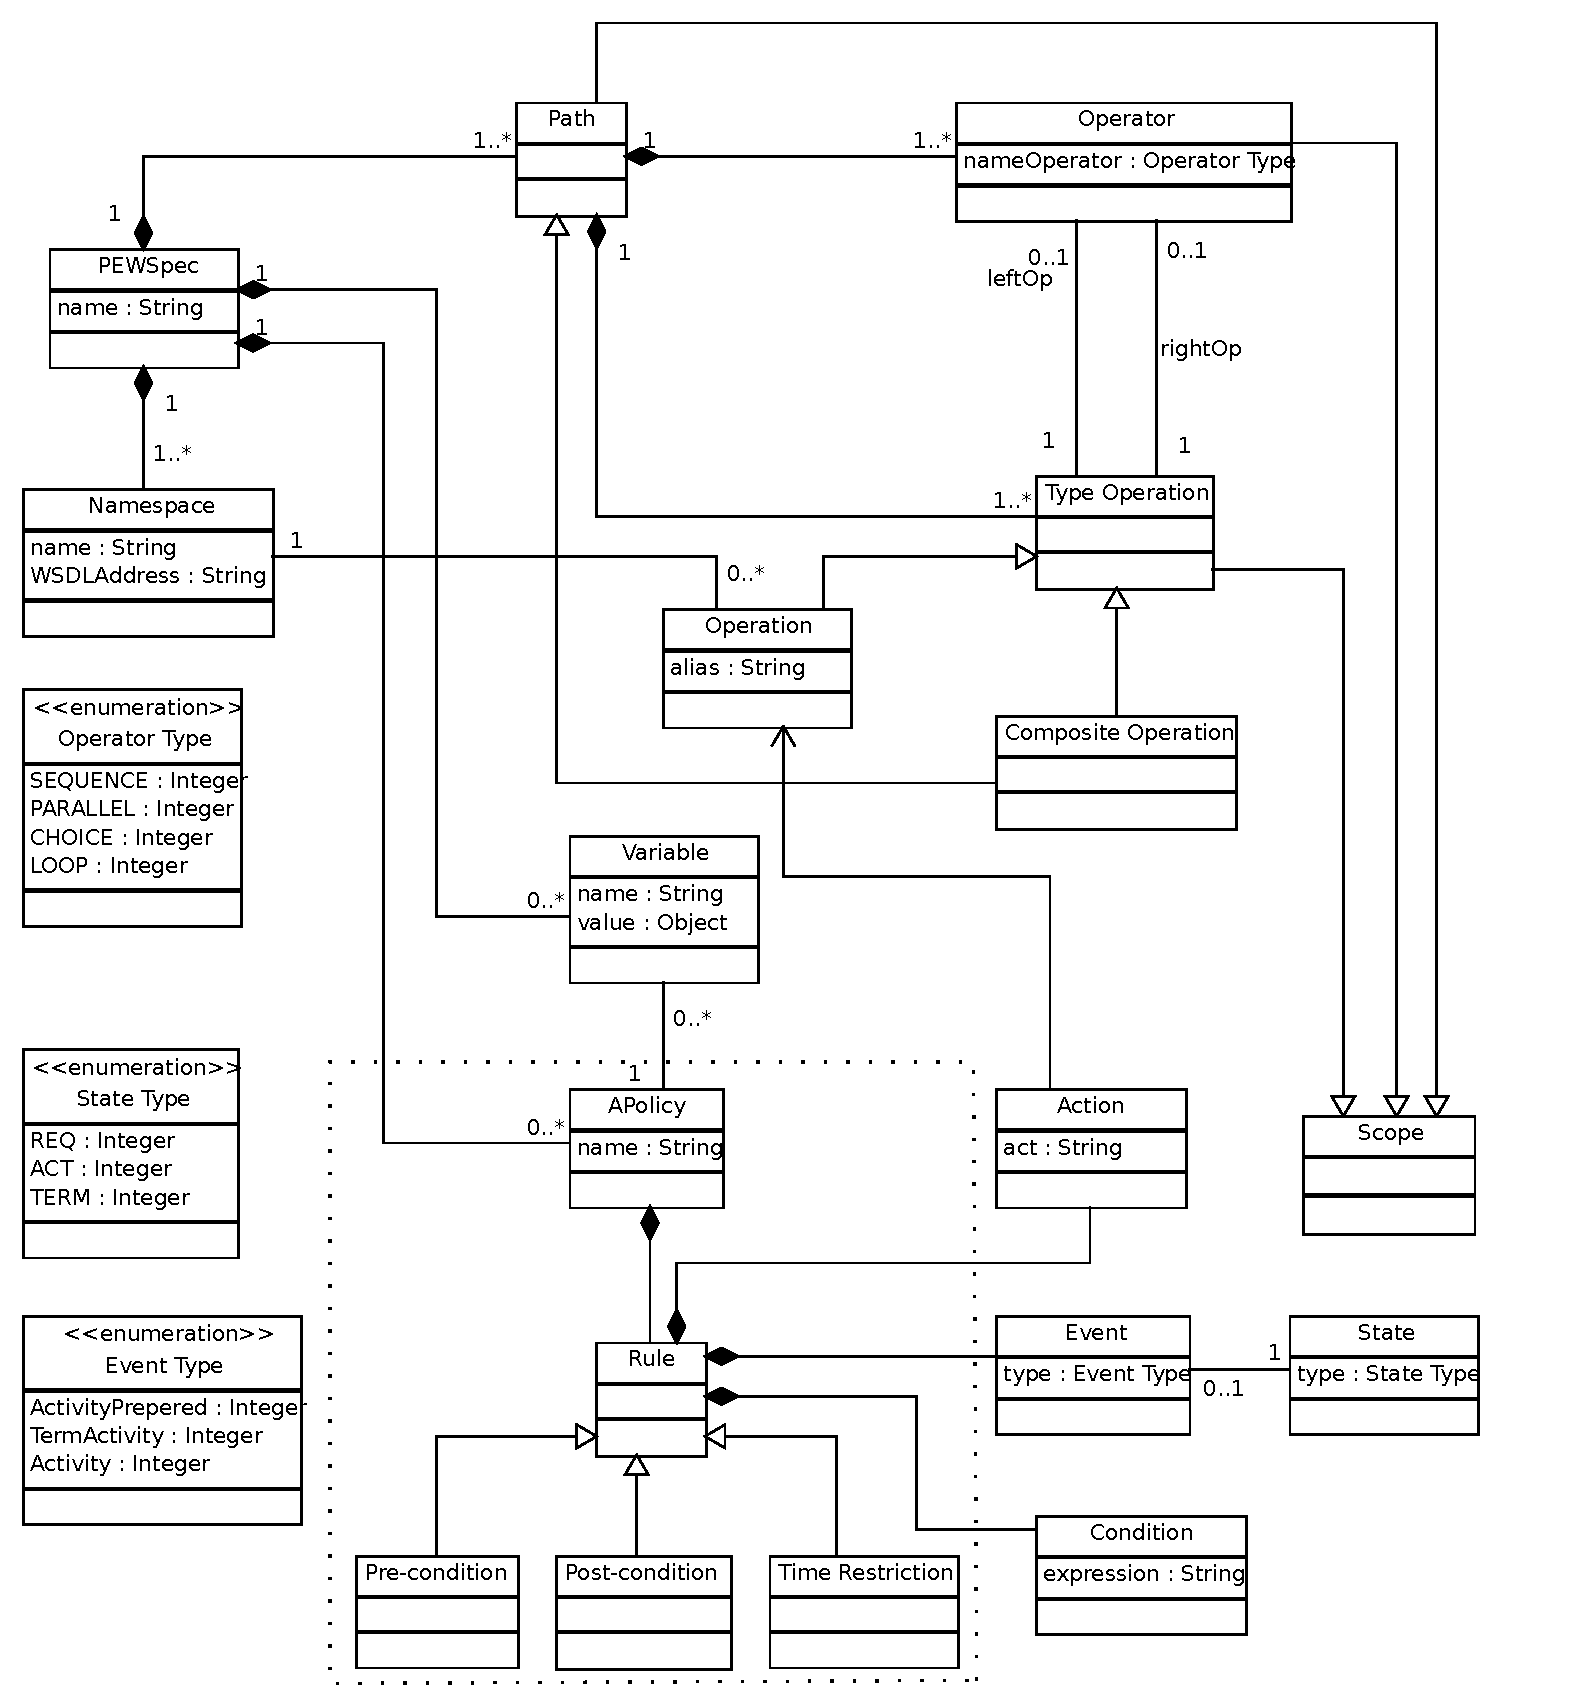
\includegraphics[width=1.0\textwidth]{figs/PEWSMetamodel}
\caption{$\pi$-{\sc Pews} Metamodel}
\label{fig:metamodel}
\end{figure}

Figure~\ref{fig:metamodel} shows that each {\sc A-Policy} is associated to a {\sc Scope} that can be either an {\sc Operation} (e.g., an authentication protocol associated to a method exported by a service),  an {\sc Operator} (e.g., a temporal constraint associated to a sequence of operators) or a {\sc Path}.  
Each {\sc A-Policy} groups a set of ECA rules with a classic semantics, i.e, {\em when an event of type E occurs, if condition C is verified then execute the action A}.  
In this way, an {\em A-policy} represents a set of reactions to be possibly executed when one or several events are notified.

Given a $\pi$-SCM model of a specific service based application (expressed according to the $\pi$-SCM meta-model), it is possible to generate its corresponding $\pi$-{\sc Pews} model. 
The following section describes the transformation rules between the $\pi$-SCM and $\pi$-{\sc Pews} meta-models.






===================================

The {\em A-policy} based service composition ($\pi$-SCM) meta-model, shown in Figure \ref{fig:e-scomposition-metamodel},
provides meta-classes to represent workflows\footnote{Workflows will be transformed into implemented service compositions.} that model  business processes.
The meta-model identifies {\sc Business Collaborators}\footnote{We use {\sc capitals} for referring to meta-model meta-classes.} and the {\sc Actions} they perform. 
Instances of this meta-model are represented as UML activity diagrams. 
In Figure~\ref{fig:e-scomposition-metamodel}  coloured boxes illustrate classes  modelling  non-functional properties and 
 white boxes represent classes modelling functional ones. 

%In the meta-model of Figure~\ref{fig:e-scomposition-metamodel}:
\begin{itemizedTrivlist}
\item A {\sc Business Collaborator} meta-class represents the classes of entities that collaborate in  business processes by performing some  required action. 
An instance of this meta-class is graphically represented as a partition in the activity diagram. 
A collaborator can be either internal or external to the system. 
When the collaborator of the business is external to the system, the attribute {\sf IsExternal}\footnote{We use the {\sf sans serif} font for referring to classes defined using a meta-model.} of the collaborator is set to \textbf{true}.

\item {\sc Action}s, a kind of {\sc ExecutableNode}, are represented in the model as a class activity instance of the meta-class Action. 
A class action represents some type of transformation or processing. 
There are two types of actions: i) a WebService (attribute Type is {\sf WS}); and ii) a simple operation called an {\sc ActivityOperation} (attribute Type is {\sc AOP}).
\begin{figure}[t]
\centering
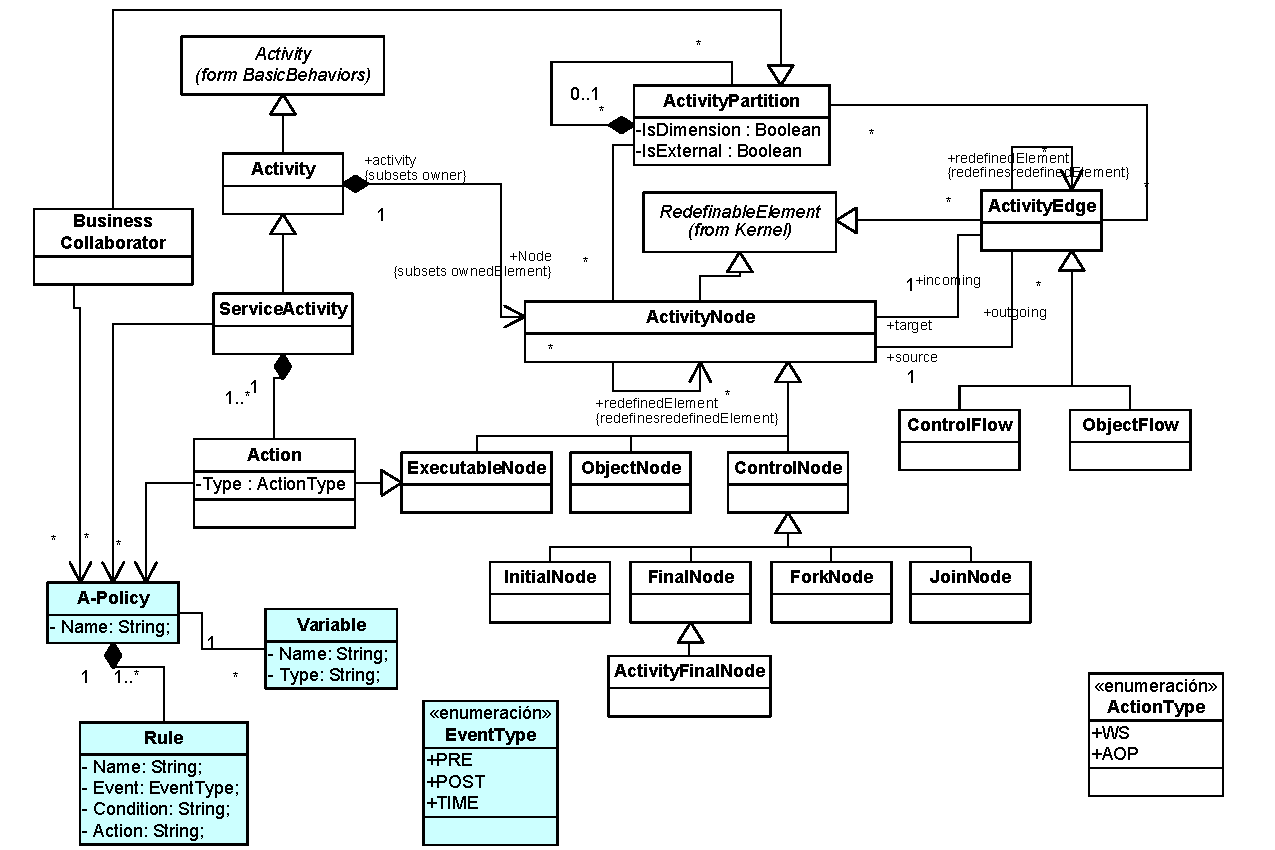
\includegraphics[width=1.0\textwidth]{figs/E-service-composition-metamodel}
\caption{$\pi$-Service Composition ($\pi$-SCM) Metamodel.}
\label{fig:e-scomposition-metamodel}
\end{figure}

\item The {\sc ServiceActivity} meta-class represents classes of composite activity types that must be carried out as part of a business service and is composed by one or more executable nodes.

\item In order to represent constraints types associated to services compositions, we extended introduced the meta-classes {\sc Rule} and {\sc A-policy} (see blue meta-classes in the $\pi$-SCM meta-model in Figure \ref{fig:e-scomposition-metamodel}).
We model non-functional constraints by using the notion of {\em A-policy}~\cite{Espinosa-Oviedo2011a,CIC:eovszmc09c}.
An {\em A-policy} is defined by attributes and rules. 
Intuitively, the conditions of each rule will be checked.
In case of no compliance, the actions defined by the rule will be performed.
The {\sc Rule} meta-class represents the types of event - condition - action rules where the {\sc Event} part represents the moment in which a constraint  will be evaluated.
An {\em A-policy} defines variables and operations that can be shared by the rules and that can be used for expressing their Event and Condition parts. 
\end{itemizedTrivlist}

\begin{figure}[t]%[htpb]
\centering
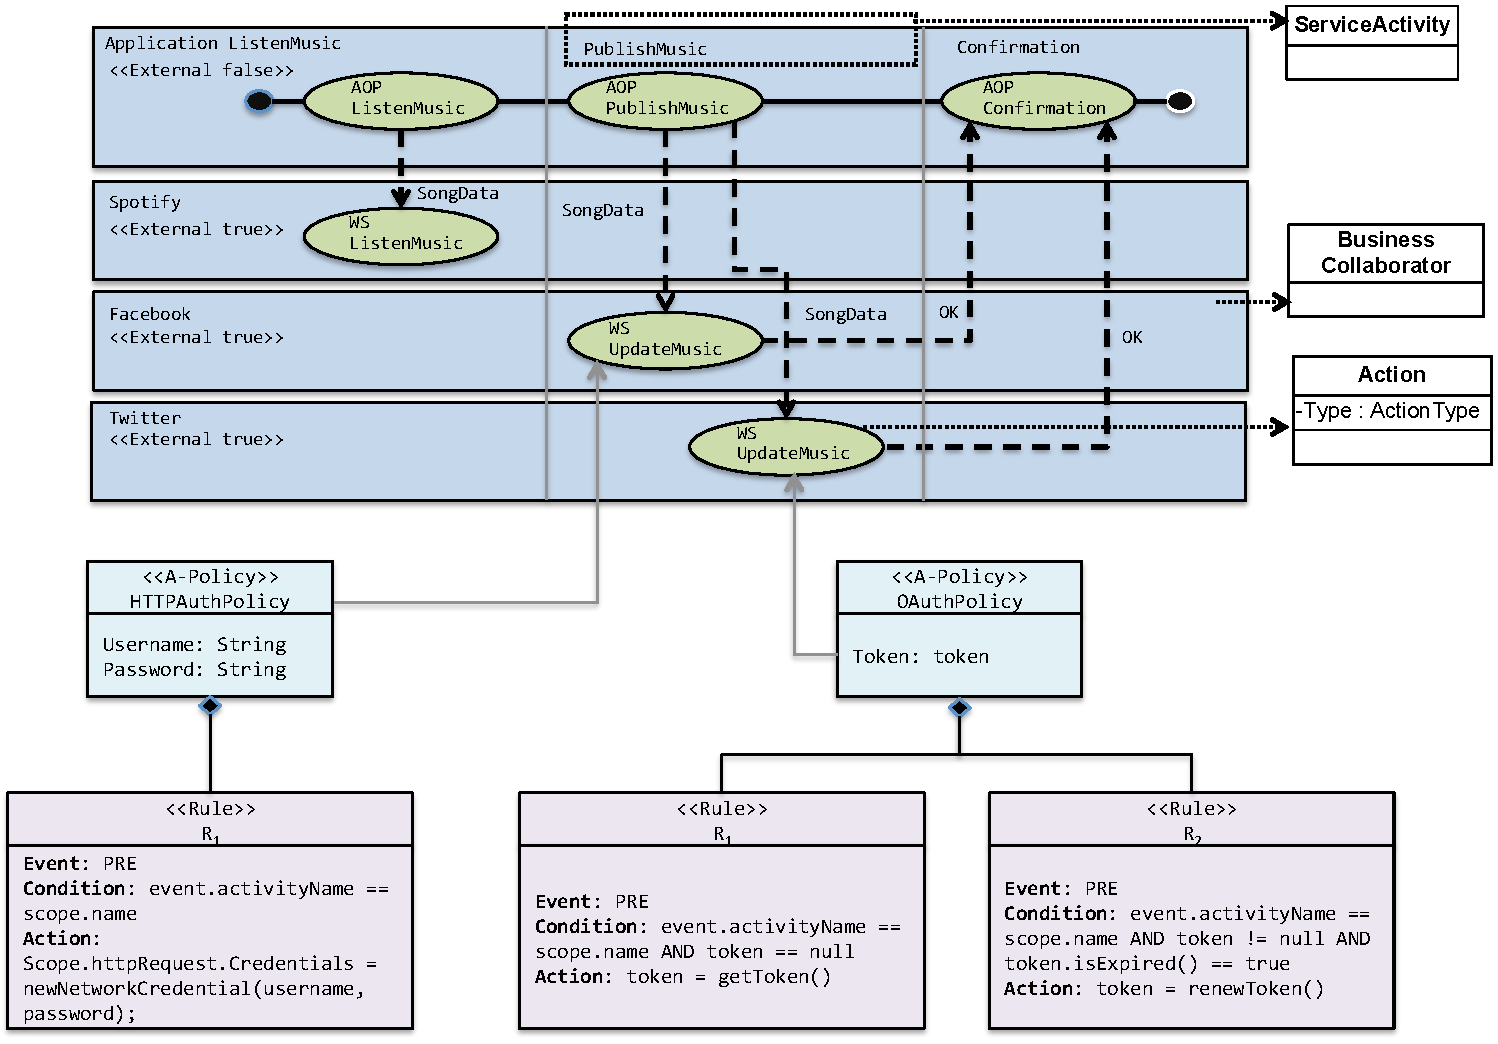
\includegraphics[width=0.95\textwidth]{figs/e-composition-model}

{\color{red}\LARGE PLACIDO: Please change the names of the boxes in accordance to the explanation --Martin}

\caption{$\pi$-SCM for the ``To publish music'' business service.}
\label{fig:servicecompositionmodel}
\end{figure}

\begin{example}[To Publish Music]\label{ex:toPublicMusic}
To illustrate the use of the $\pi$-Service Composition Meta-model, we define a model for the ``To Publish Music'' scenario (Figure \ref{fig:servicecompositionmodel}). 
In this model, there are three external business collaborators ({\em Spotify, Twitter} and {\em Facebook}).
% \footnote{We use {\em italics} to refer to concrete values of the classes of a model that are derived from the classes of a meta-model.}). 
The model also shows the business process of the application that consists of three service activities: {\em Listen Music}, {\em Publish Music} and {\em Confirmation}. 
Note that  the activity {\em Publish Music} calls the actions of two service collaborators namely {\em Facebook} and {\em Twitter}.
Both {\em Facebook} and {\em Twitter} services require authentication protocols in order to execute methods that will read and update the user space. 
%A call to such services must be part of the authentication protocol required by these services.
In the example we  associate two authentication policies, one for the open authentication protocol, represented by the class {\sf\small OAuthPolicy} at {\em Twitter}, that will be associated to the activity  {\sf\small UpdateTwitter} (see Figure \ref{fig:servicecompositionmodel}). 
In the same way, the {\em Facebook} class {\sf\small HTTPAuthPolicy}, for the http authentication protocol will be associated to the activity {\sf\small UpdateFacebook}.

{\sf\small OAuthPolicy} will implement the open authentication protocol.
The {\em A-policy} {\sf\small OAuthPolicy} has a variable {\sf\small Token} that will be used to store the authentication token provided by the service.
This variable is imported through the library {\sf\small OAuthPolicy.Token}. 
The A-policy {\sf\small OAuthPolicy} defines two rules, both can be triggered by events of type {\sf\small ActivityPrepared}: (R$_1$): If no token has been associated to the variable {\sf\small token}, then a token is obtained ; and (R$_2$): if the token has expired, then it is renewed. 
Notice that the code in the actions profits from the imported {\sf\small OAuthPolicy.Token} for transparently obtaining or renewing a token from a third party.

{\sf\small HTTPAuthPolicy} implements the HTTP-Auth protocol. 
The A-policy imports an http protocol library and it has two variables {\sf\small username} and {\sf\small password}.  
The event of type {\sf\small ActivityPrepared} is the triggering event of the rule {\sf\small R$_1$}. 
On the notification of an event of that type, a credential is obtained using the username and password. 
\hfill\openbox
\end{example}

We propose the use of rules and policies to model and associate non-functional properties to service compositions.
These artifacts will be used to generate the actual programs that will implement the application:
Once the $\pi$-Service Composition Model has been defined, then it can be transformed into a lower level model (in our case, $\pi$-PEWS) that gives support to code generation. 
The $\pi$-PEWS  meta-model is described in the next section. 


%..--..--..--..--..--..--..--..--..--..--..--..--..--..--..--..--..--..--..--..--..--..--..--..--..--..--..--..--..--..--..--..
\subsubsection{$\pi$-{\sc Pews}  meta-model}\label{sec:pewsmetamodel}
%..--..--..--..--..--..--..--..--..--..--..--..--..--..--..--..--..--..--..--..--..--..--..--..--..--..--..--..--..--..--..--..


